\documentclass{jarticle}
\usepackage{robomech}

\usepackage{mathrsfs}
\usepackage{bm}
\usepackage[dvipdfmx]{graphicx}
\usepackage{enumerate}

\begin{document}
\makeatletter
\title{未知障害物環境に対応するための\\モンテカルロ自己位置推定における観測範囲の選択}
{―まだ決まってない―}
{Observation Range Selection in Monte Carlo localization for Unknown Obstacle Environments}
{-Not decided yet.-}

\author{
\begin{tabular}{ll}
 ○学\hspace{1zw} 池邉龍宏(千葉工大)& 正\hspace{1zw}林原靖男\hspace{1zw} (千葉工大)\\
 \hspace{1zw}正\hspace{1zw}上田隆一(千葉工大)\\
 % ※協賛・後援団体の会員資格で発表される場合は「正・学」は不要です。
 \end{tabular}
 % &\\
 \vspace{1zh} \\
 \begin{tabular}{l}
{\small Tatsuhiro IKEBE, Chiba Institute of Technology, 
 }\\
 {\small Yasuo HAYASHIBARA, Chiba Institute of Technology}\\
 {\small Ryuichi UEDA, Chiba Institute of Technology}\\
\end{tabular}
}
\makeatother

\abstract{ \small 
Not decided yet.
}

\date{} % 日付を出力しない
\keywords{Autonomous mobile robots, Navigation, LiDAR Localization, MCL, Unknown Obstacle}

\maketitle
\thispagestyle{empty}
\pagestyle{empty}


\section{緒言}%===========================

近年、自律移動ロボットの自己位置推定手法として、 Monte Carlo localization(MCL)\cite{MCL}
がよく用いられる。MCLは、ロボットのとりうる姿勢
$\mathcal{X}$$=$$\{\bm{x}=(x, y, \Theta)^T | x \in [x_{min}, x_{max}], y \in [y_{min}, y_{max}] ,\theta \in [-\pi, \pi)] )\}$
を多数のパーティクルで近似し、
予測更新、観測更新、リサンプリングにより、推定した姿勢$\bm{x}$${ = (x, y, \Theta)}$を出力とするアルゴリズムである。
また、MCLのアルゴリズムで使用されるパーティクルフィルタは、
他の自己位置推定用フィルタと比較すると、
パーティクルの数によって計算量が増加してしまうが、
非線形なモデルにおいても推定が可能であり、事後分布をパーティクルとして
表せれることからマルチモーダルな分布を求めることができる利点がある。

しかし、MCLは、静的環境とマルコフ性を仮定しており、
環境に存在する未知障害物の対策は出来ていない。
そのため、未知障害物が存在する環境では、自己位置推定が破綻しやすい。
ここでいう未知障害物とは、ロボットが持っている地図(静的環境)以外の障害物のことである。

そのような環境の例としては、つくばチャレンジ\cite{つくばチャレンジ}が挙げられる。つくばチャレンジというのは、
実際に人や自動車が通る横断歩道、公園において、ロボットを約2km自律走行させる技術チャレンジである。
図\ref{fig: つくばチャレンジ人混み}は、つくばチャレンジのスタート地点である。

図\ref{fig: つくばチャレンジ人混み}のような人混みで溢れる環境は、ロボットが持っている地図とLiDAR等の
センサから得られるデータの照合を誤る可能性が高い。
これは、MCLの観測更新において、地図に載っている静的障害物ではなく、
その近くにある未知障害物が地図に載っている静的障害物であるとしてしまうことに起因する。
照合を誤った場合、結果的にそれが原因で自己位置推定が破綻する。

未知障害物による自己位置推定の破綻に対応するための、富沢ら\cite{富沢}、赤井ら\cite{赤井}の研究がある。
富沢ら\cite{富沢}は、測域センサで観測したローカル地図と環境地図を
二値のグリッドマップで表現し、各パーティクル位置における画像の不一致ピクセル量に基づいたパー
ティクルの尤度評価方法を提案した。また、この手法において、動的環境でロバストに自己位置を
推定し、経路に沿って安全に走行できることを証明した。
赤井ら\cite{赤井}は自己位置とセンサ観測のクラスを同時推定す
る方法を提案した。この手法により、地図上にある観測であるか判別できるようにした。
これを利用し、地図上に存在する障害物から得られている
センサ観測のみをパーティクルの観測更新に使用することで、
動的障害物やランドマークの移動・除去に関する環境変化に対して、
頑健に位置推定ができることを確認した.

これらの従来研究の未知障害物を観測に含めないことにより自己位置推定の破綻を防ぐという
考えから、パーティクルごとに観測範囲を持たせるというアイデアを得た。
そこで、本稿では、そのアイデアをMCLに実装し、実装後のMCLの性能について評価を行う。
2章では、未知障害物対策を実装したMCL、3章では実装したMCLの性能評価を行うための実験、
4章では実験結果から性能評価を行い、最後に結言で本稿をまとめる。

\begin{figure}[h!]
  \centering
   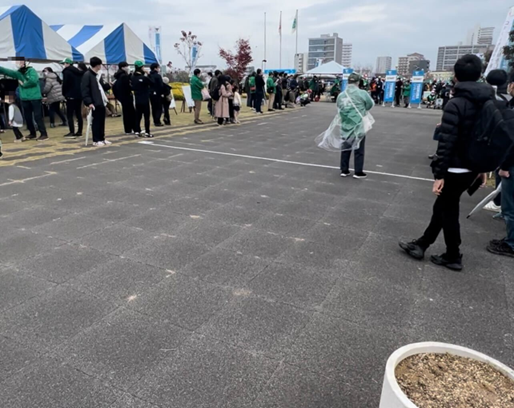
\includegraphics[height=50mm]{fig/hitogomi.png}
   \vspace*{-4mm}
   \caption{Crowds at the start of the Tsukuba Challenge 2022}
   \label{fig: つくばチャレンジ人混み}
 \end{figure}

\section{手法}%===========================

主なアルゴリズムの流れを図\ref{fig: つくばチャレンジ人混み}に示す。
初期化の部分で各パーティクルごとにランダムな観測範囲を付与する。
次に、動作モデルと観測モデルによる更新、リサンプリングを行うことで、
未知障害物が含まれていないような観測範囲をMCLのアルゴリズムによって求める。


\subsection{各パーティクルの初期化}

各パーティクルの初期化時に各パーティクルに対して、
ランダムな観測を与える。
ランダムな観測とは、360°のうちの、ある角度分を観測としたものである。

\subsection{動作モデル}

動作モデルは、MCLのアルゴリズム通りである。

\subsection{観測モデル}

観測モデルでは、各パーティクルの入力として、生の観測を受け取る。
観測を受け取り、各パーティクルはランダムな観測範囲を元に観測を間引く。
間引いた観測を元に尤度場から、そのパーティクルの尤度を求める。
尤度をかけ合わせたものをそのパーティクルの重みとする。

\subsection{リサンプリング}

リサンプリングでは、パーティクルの重みの正規化を行う。
また、1割程度の各パーティクルに対してランダムな観測範囲を再付与させる。
これは、各パーティクルがある観測範囲を選択し続ける問題を避けることが目的である。

\section{実験}%===========================

\subsection{実験環境}

2節で説明した手法を実装し、その効果の検証をするためにシミュレータ環境を用いた。
今回、使用した環境を図\ref{fig: 人混みガゼボ}、
\ref{fig: つくばチャレンジ人混みシミュレータ}に示す。
この環境は、図\ref{fig: つくばチャレンジ人混み}のつくばチャレンジでの人混みの環境を模したものである。
環境には、人型や箱型の未知障害物を多く配置した。全ての未知障害物は速度0[m/s]である。

今回使用したPCの環境を表\ref{table: PCの環境}に示す。
シミュレータのソフトウェアとしてGazebo、ナビゲーションのシステムとしてROS Noeticを使用する。

実験に用いるシミュレータ内のロボットは、図\ref{fig: raspicat}のような差動二輪型のロボットである。
ロボットおよび搭載しているセンサの性能について、表\ref{table: ロボットおよび搭載しているセンサの性能}に示す。
図\ref{fig: raspicat}には示されていないが、1mの高さに観測用のセンサとして、2D LiDARを搭載している。
2D LiDARの観測範囲は360°であり、角度分解能は1°である。
ロボットの最高速度は、3[m/s]である。

\begin{table}[hbtp]
  \caption{experimental environment}
  \label{table: PCの環境}
  \centering
  \begin{tabular}{lcr}
    \hline
    CPU & Core™ i9-12900K × 24 \\
    GPU & GeForce RTX 2060 \\
    Ubuntu & 20.04 \\
    ROS  & Noetic \\
    Gazebo  &  9.0 \\
    \hline
  \end{tabular}
\end{table}

\begin{table}[hbtp]
  \caption{performance of the robot and on-board sensors}
  \label{table: ロボットおよび搭載しているセンサの性能}
  \centering
  \begin{tabular}{lcr}
    \hline
    ロボットの最高速度 & 3[m/s] \\
    2D LiDARの取り付け高さ & 1[m] \\
    2D LiDARの観測範囲 & 360° \\
    2D LiDARの角度分解能 & 1° \\
    \hline
  \end{tabular}
\end{table}

\begin{figure}[htbp]
  \centering
   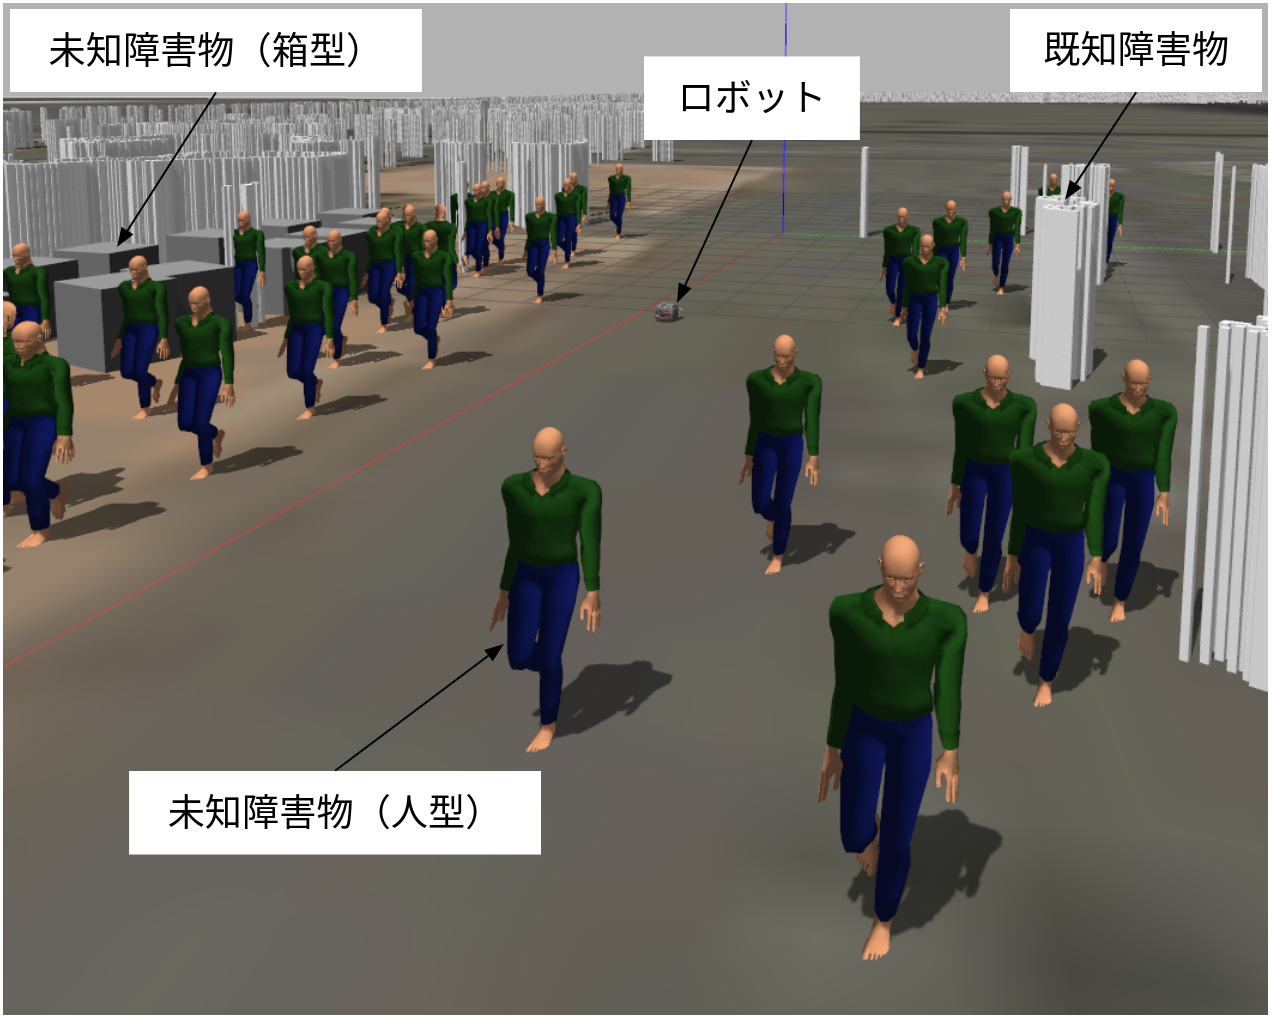
\includegraphics[height=50mm]{fig/hitogomi_gazebo.png}
   \vspace*{-4mm}
   \caption{Where localization has broken down}
   \label{fig: 人混みガゼボ}
\end{figure}

\begin{figure}[htbp]
  \centering
   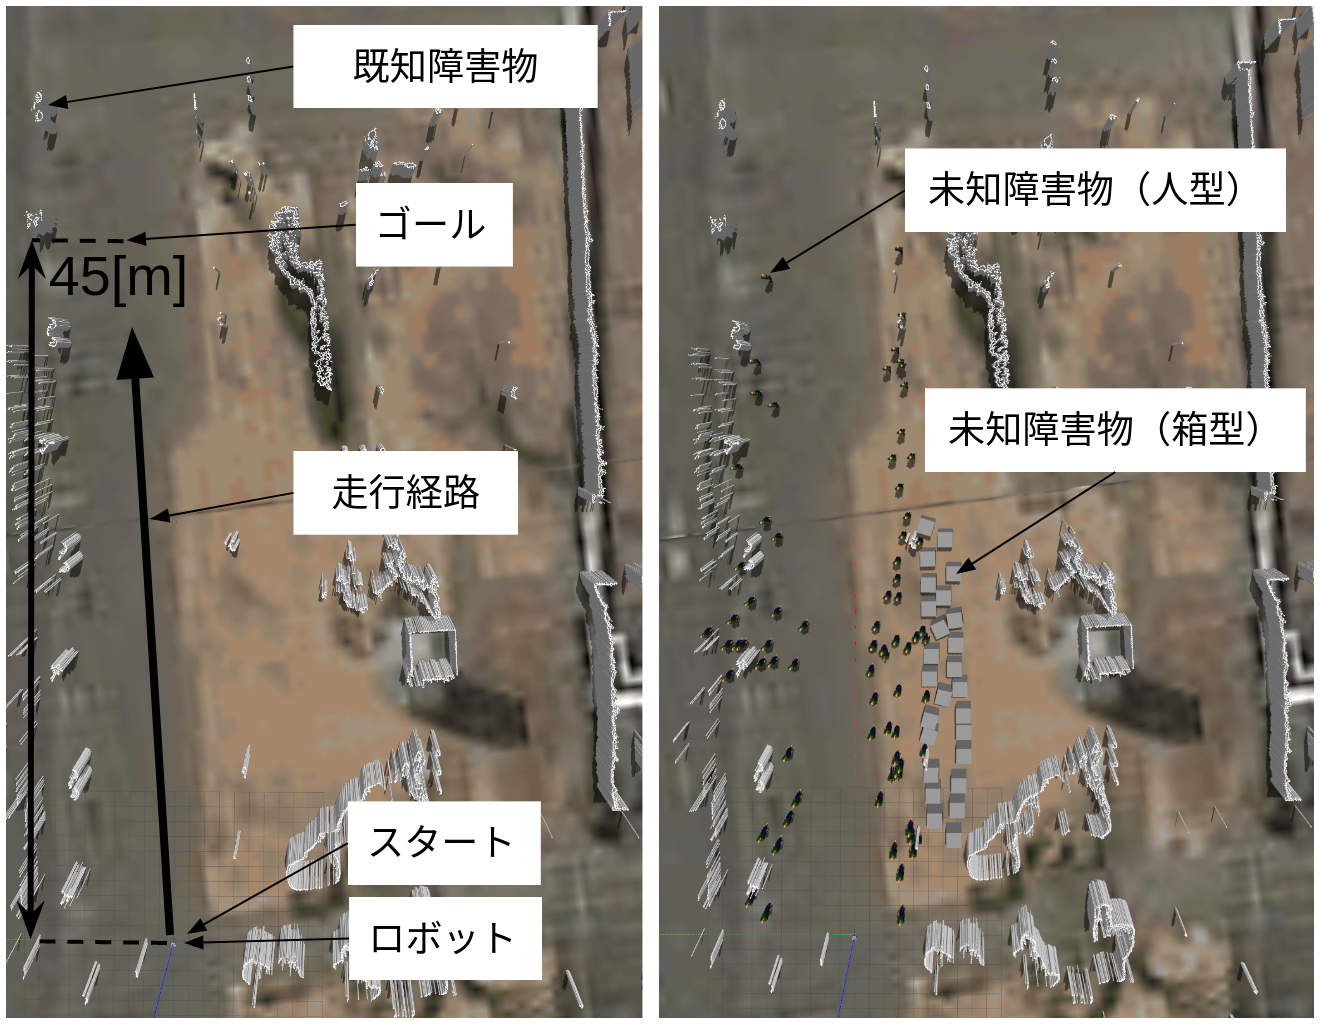
\includegraphics[height=70mm]{fig/environment_comparison.png}
   \vspace*{-4mm}
   \caption{A simulator that mimics the crowds at the start of Tsukuba Challenge 2022}
   \label{fig: つくばチャレンジ人混みシミュレータ}
\end{figure}

\begin{figure}[htbp]
  \centering
   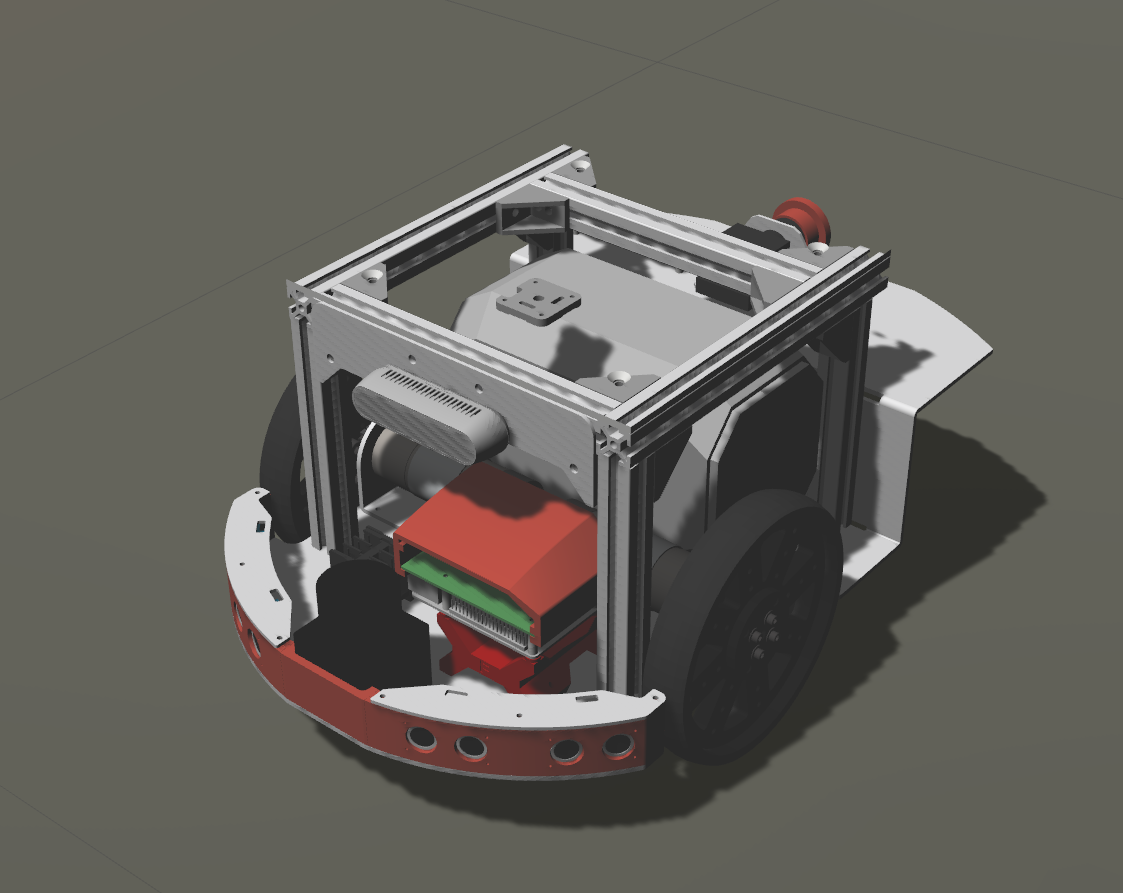
\includegraphics[height=50mm]{fig/raspicat_gazebo.png}
   \vspace*{-4mm}
   \caption{Where localization has broken down}
   \label{fig: raspicat}
\end{figure}

\subsection{実験方法}

実験方法は以下のとおりである。
\noindent
\begin{enumerate}[A]
  \item スタートからゴールまでオンラインでロボットのナビゲーションをする
  \item 事前にジョイスティックでロボットをスタートからゴールまで動かす。
        その間、得られた観測情報等を記録したデータを後から再生し、オフラインで自己位置推定をする。
\end{enumerate}
\noindent
スタートとゴールは、それぞれ図\ref{fig: スタートからゴールまでナビゲーション}
に示された位置である。

今回の実験の評価項目は、以下のとおりである。
\begin{itemize}
  \item スタートからゴールまでの完走率(実験方法A)
  \item スタートからゴールまで走行したときの真値との比較(実験方法B)
  \item パーティクルの観測更新に最も使用された観測(実験方法A)
  \item 計算時間の増減(実験方法A)
\end{itemize}

\subsection{実験目的}

色々なパターンのパーティクルの条件で実験を行う。
パーティクルの条件については、後述で説明する。
3.2節で説明した実験の評価から良さそうなパーティクルの条件とその性能について求めることが、今回の実験目的である。

\section{実験結果}%===========================

\subsection{完走率}

表\ref{table:完走率}に、実験方法Aにより求めた、各パーティクルの条件での完走率を示す。
結果からは、観測範囲が狭くなるほど完走率が大きくなっていることがわかる。

\begin{table}[htbp]
  \caption{completion rate under certain particle conditions}
  \label{table:完走率}
  \begin{tabular}{|c|r|r|r|} \hline
  条件番号 & パーティクル数 & 観測範囲  & 完走確率 \\ \hline \hline
  \textcircled{\scriptsize 1} & 3000 & 0° & 0 \\ \hline
  \textcircled{\scriptsize 2} & 3000 & 10° & 0.52 \\ \hline
  \textcircled{\scriptsize 3} & 3000 & 360° & 0 \\ \hline
  \textcircled{\scriptsize 4} & 10000 & 0° & 0 \\ \hline
  \textcircled{\scriptsize 5} & 10000 & 1° & 0.28 \\ \hline
  \textcircled{\scriptsize 6} & 10000 & 10° & 0.54 \\ \hline
  \textcircled{\scriptsize 7} & 10000 & 45° & 0.04 \\ \hline
  \textcircled{\scriptsize 8} & 10000 & 90° & 0 \\ \hline
  \textcircled{\scriptsize 9} & 10000 & 360° & 0 \\ \hline
  \textcircled{\scriptsize 10} & 10000 & 1$\sim$15° & 0.54 \\ \hline
  \end{tabular}
\end{table}

各パーティクルの条件において、自己位置推定が破綻した場所を
図\ref{fig: 失敗箇所}に示す。
\textcircled{\scriptsize 3}\textcircled{\scriptsize 5}\noindent
\textcircled{\scriptsize 8}\textcircled{\scriptsize 9}\noindent
の条件は、スタートから12mあたり、
\textcircled{\scriptsize 2}\textcircled{\scriptsize 6}\noindent
\textcircled{\scriptsize 7}\textcircled{\scriptsize 10}\noindent
の条件は、スタートから30mのあたりで
自己位置推定が破綻することがあった。
\textcircled{\scriptsize 1}\textcircled{\scriptsize 4}\noindent
は観測範囲が0であるため、推定値が真値に対して徐々にずれていった。
ゴール地点に到達した時には20mもの誤差になった。

\begin{figure}[htbp]
  \centering
   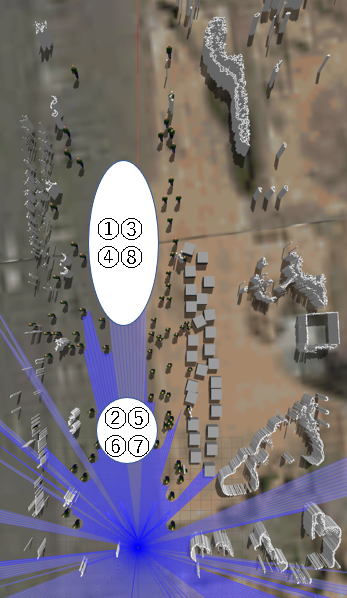
\includegraphics[height=100mm]{fig/failure_location.png}
   \vspace*{-4mm}
   \caption{Where localization has broken down}
   \label{fig: 失敗箇所}
\end{figure}

\subsection{自己位置推定の誤差}

図\ref{fig: plot}に、実験方法Bにより求めた、
真値(reference)に対する各パーティクルの条件での
自己位置推定値の誤差を示す。
まず、xy平面上に真値と自己位置推定をプロットしたものを見ると、
条件
\textcircled{\scriptsize 3}\textcircled{\scriptsize 7}\noindent
\textcircled{\scriptsize 8}\textcircled{\scriptsize 9}\noindent
の場合、スタートから約10mの場所から自己位置の推定誤差が大きくなり、自己位置推定破綻を起こした。
条件
\textcircled{\scriptsize 1}\textcircled{\scriptsize 4}\noindent
の場合、スタートから約19mの場所から自己位置の推定誤差が大きくなり、自己位置推定破綻を起こした。
条件
\textcircled{\scriptsize 2}\textcircled{\scriptsize 5}\noindent
\textcircled{\scriptsize 6}\textcircled{\scriptsize 10}\noindent
は、スタートから約15~20mの場所から自己位置の推定誤差が大きくなり始めたが、
20m以降は一定の誤差のままゴールまで到達した。
中でも条件
\textcircled{\scriptsize 5}\noindent
の誤差が小さいように見える。

xy平面上に真値と自己位置推定をプロットしたものの中でも
自己位置の推定誤差が小さかった4つの条件
\textcircled{\scriptsize 2}\textcircled{\scriptsize 5}\noindent
\textcircled{\scriptsize 6}\textcircled{\scriptsize 10}\noindent
において、真値に対する自己位置推定値のユークリッド誤差、横誤差、縦誤差
をプロットした。
4つの条件の中でも、条件
\textcircled{\scriptsize 2}\textcircled{\scriptsize 5}\noindent
の誤差が小さいように見える。
しかし、誤差が小さいといっても、それぞれの条件において、
最大で横誤差が0.4m、縦誤差が0.8m、ユークリッド誤差が0.8mもあるときがある。

\begin{figure}[htbp]
  \begin{center}
  \begin{tabular}{cc}
  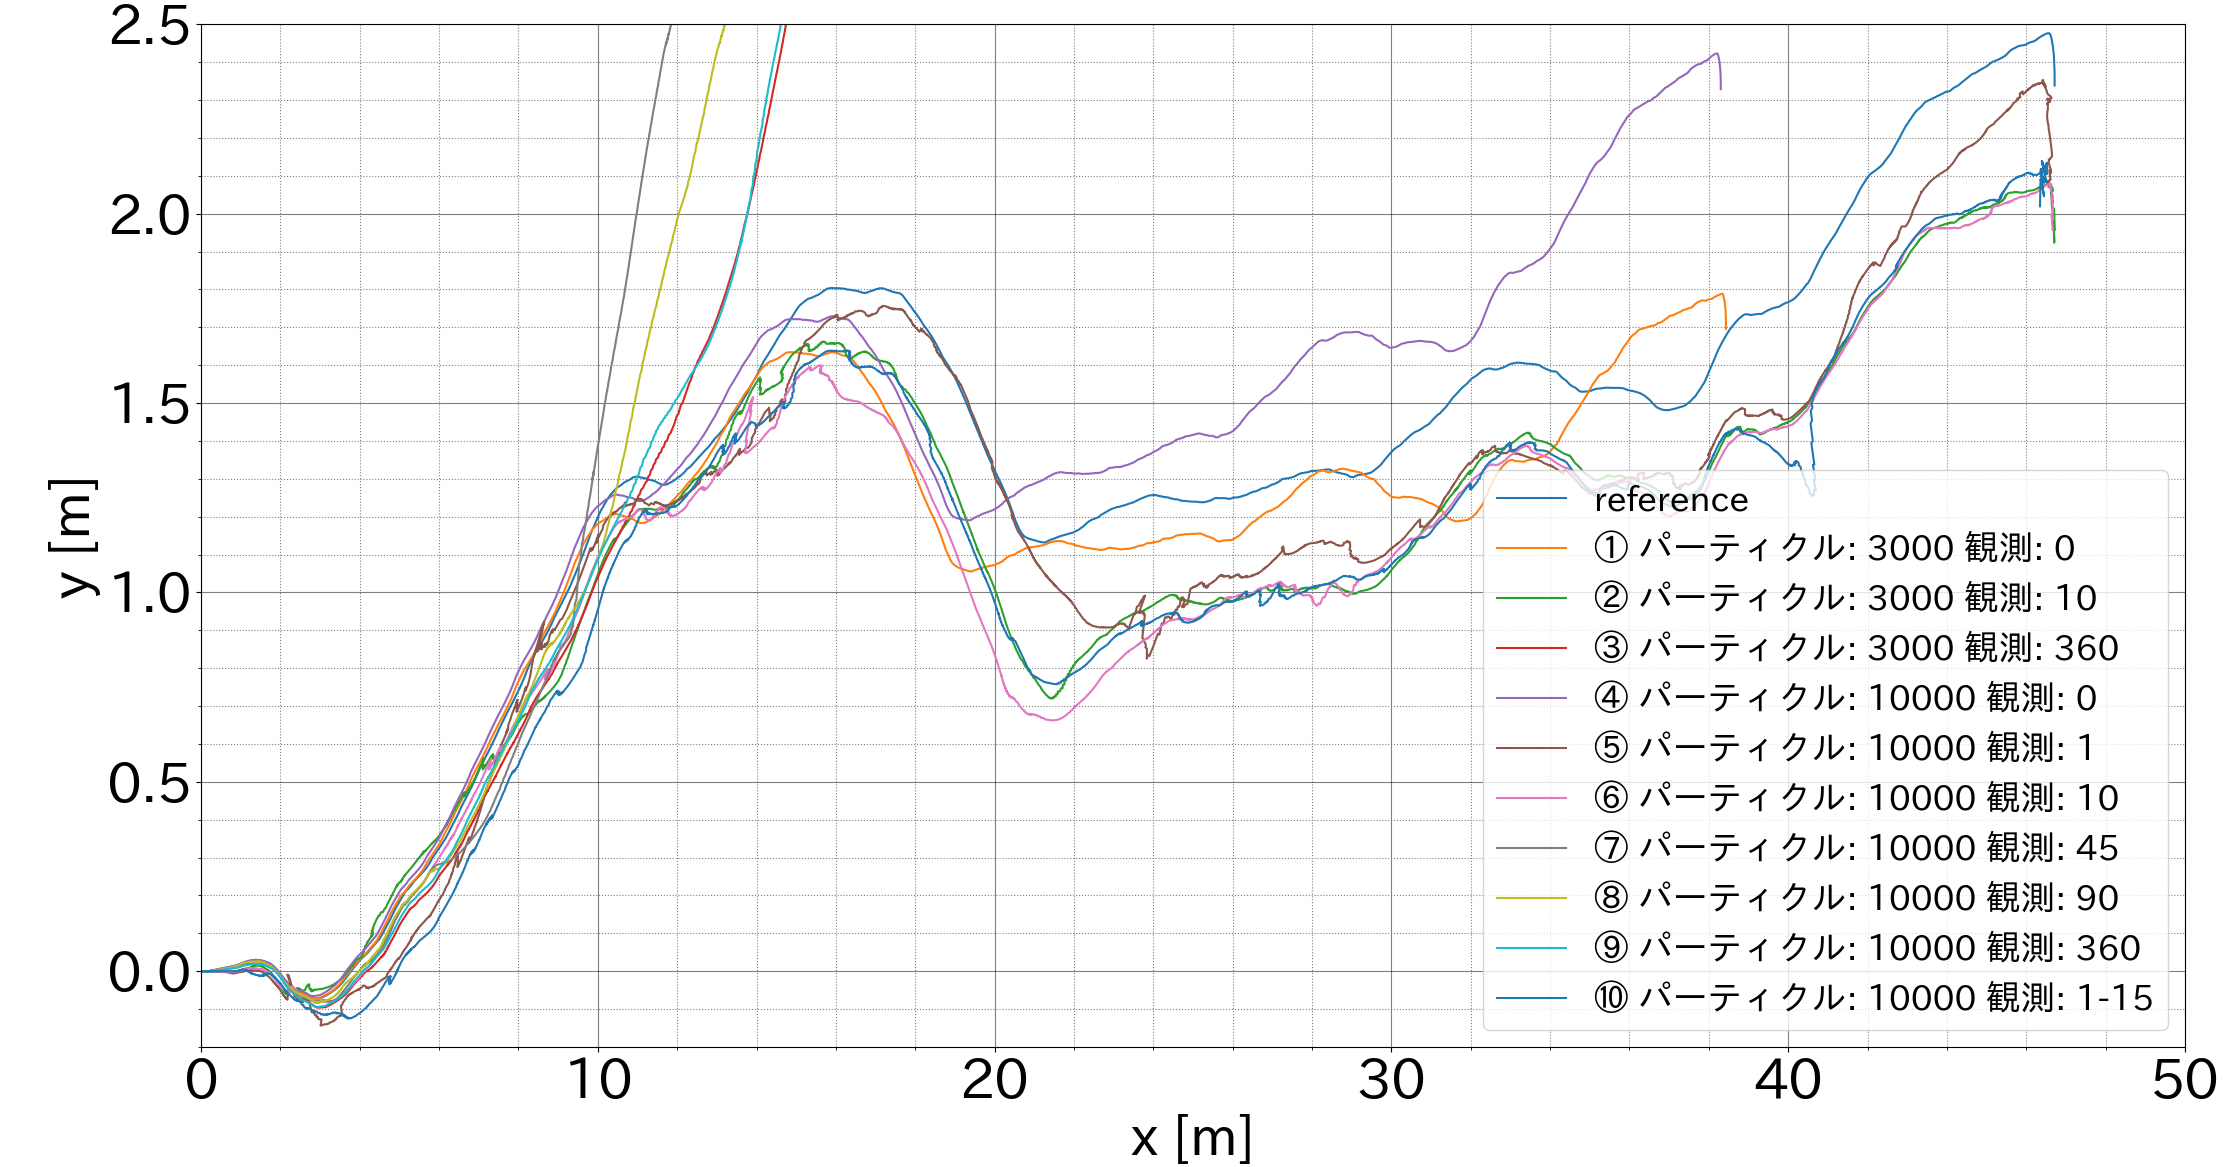
\includegraphics[height=48mm]{fig/x_y.png} \\
  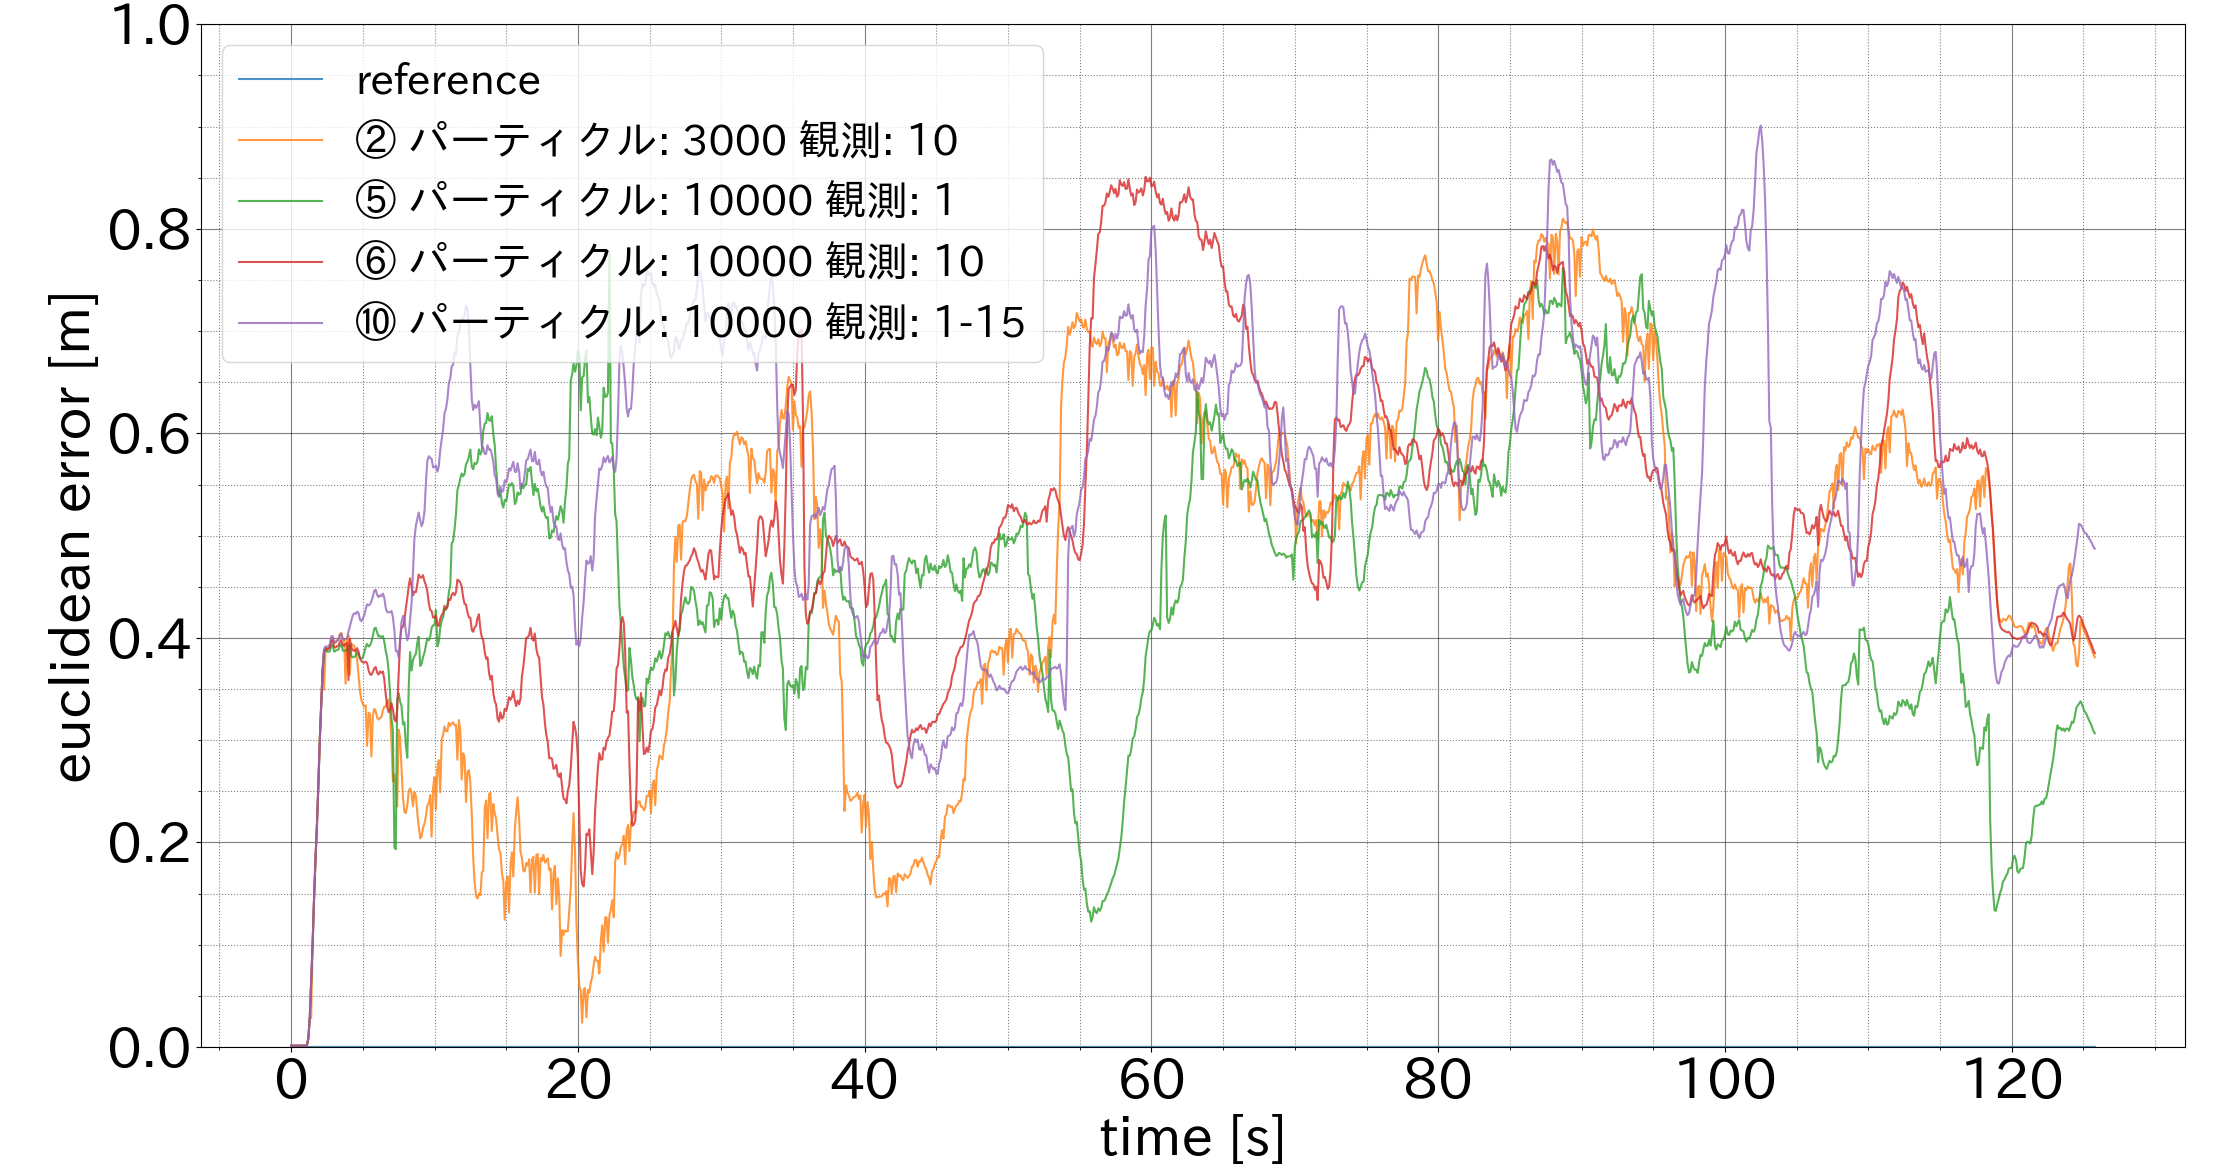
\includegraphics[height=48mm]{fig/euclidean_error.png} \\
  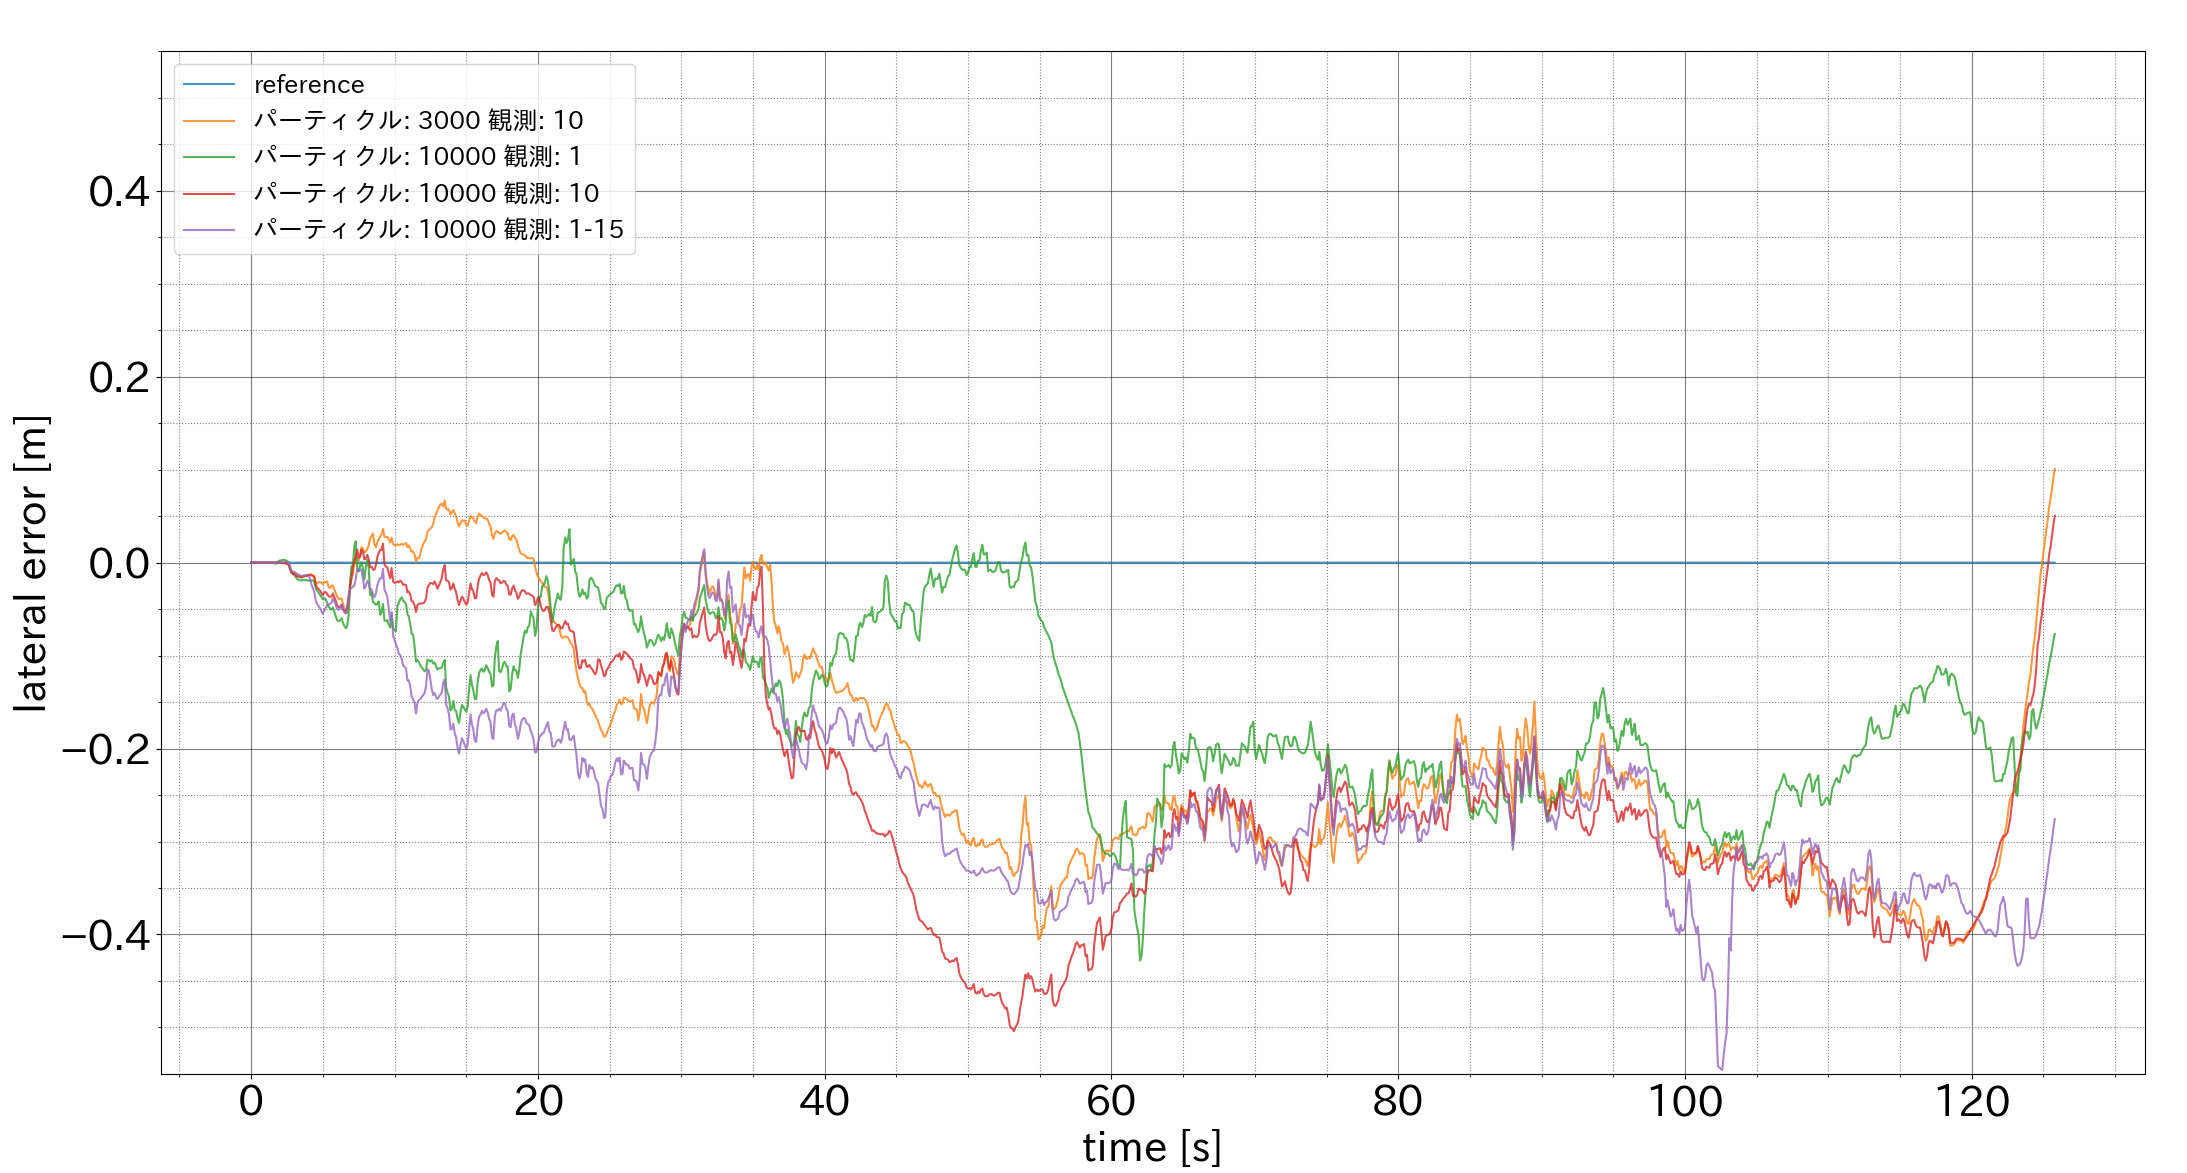
\includegraphics[height=48mm]{fig/lateral_error.png} \\
  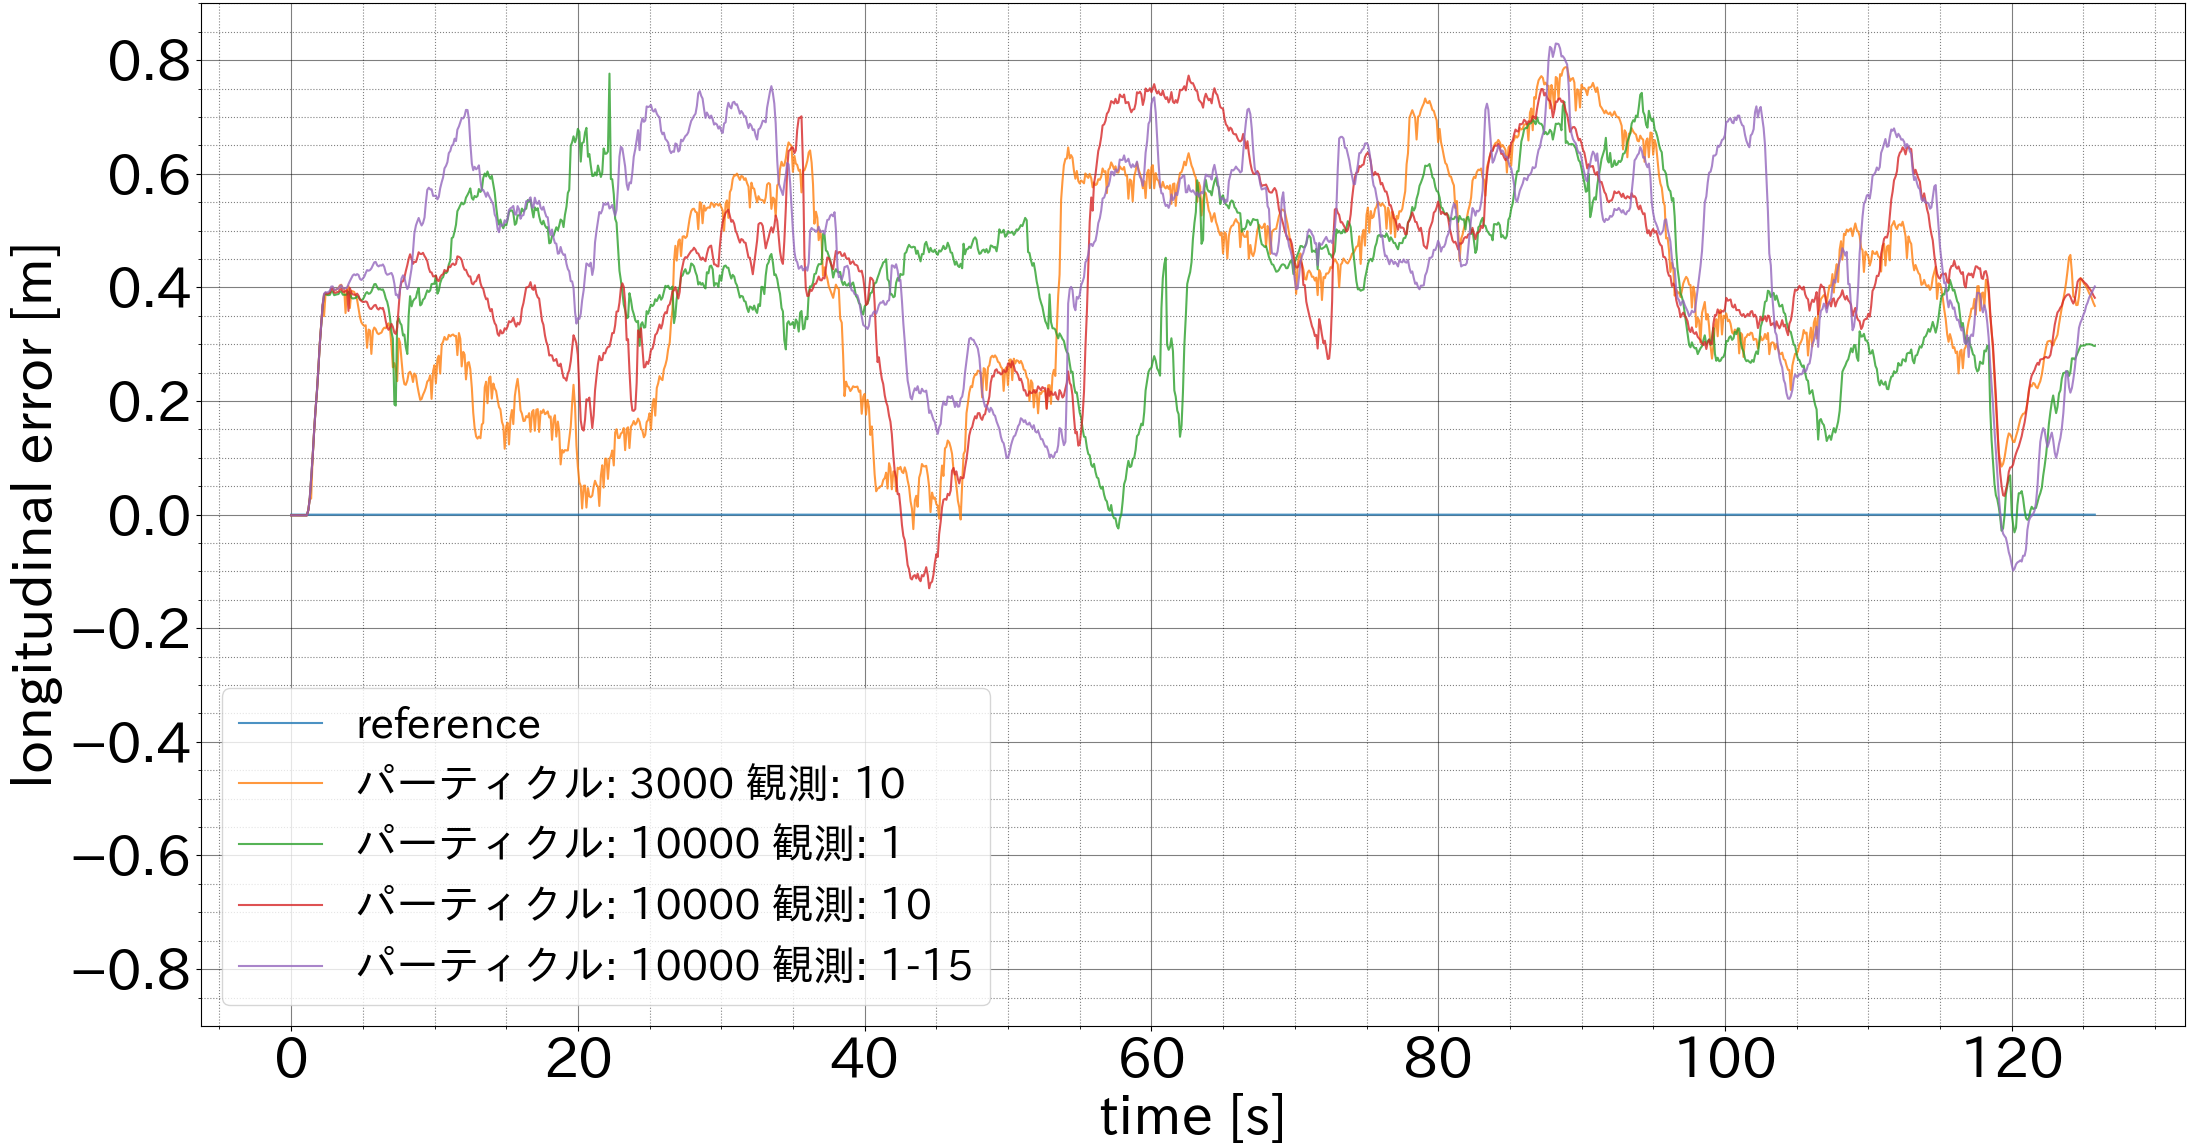
\includegraphics[height=45mm]{fig/longitudinal_error.png} 
  \end{tabular}
  \caption{
    Plot the true value and the self-estimated position value,
     and the lateral direction and the longitudinal 
    direction and Euclidean error with respect to the true value.}
  \label{fig: plot}
  \end{center}
\end{figure}

\subsection{手法を実装したMCLで使用されている観測範囲}

\begin{figure}[t]
  \centering
   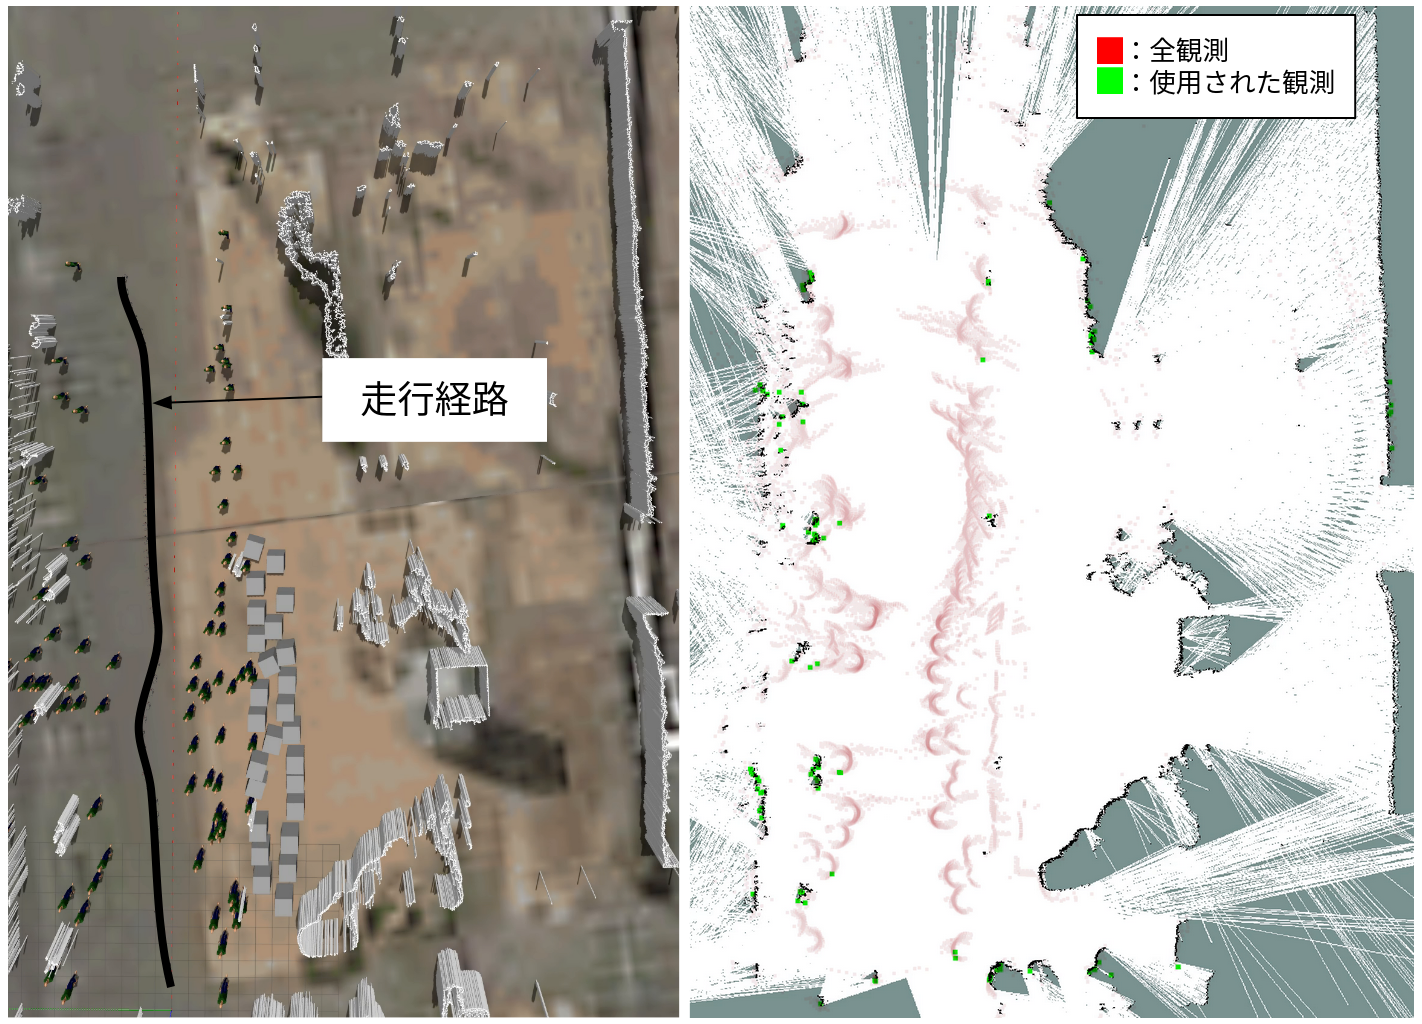
\includegraphics[height=70mm]{fig/particle_1000_observation_1_mcl.png}
   \vspace*{-4mm}
   \caption{The robot navigates from the start to the goal.}
   \label{fig: スタートからゴールまでナビゲーション}
\end{figure}

\section{結言}%===========================


\footnotesize
\begin{thebibliography}{99}

\bibitem{MCL}

\bibitem{つくばチャレンジ}

\bibitem{富沢}

\bibitem{赤井}

\end{thebibliography}

\normalsize
\end{document}
